\documentclass[a4paper, 12 pt]{article}

\usepackage{graphicx, float}
\usepackage{lmodern}
\usepackage[french]{babel}
\usepackage[T1]{fontenc}
\usepackage[utf8]{inputenc}
\usepackage{enumitem, pifont}
\usepackage{amsmath, amsfonts,amssymb} 

\title{\LARGE \textbf{LES VUES MULTIPLES D'UN SOLIDE}}
\author{MATH\'EMATHIQUES 5P}
\date{\today}
\setlist[itemize, 1]{label ={\ding{248}}, itemsep = \baselineskip}


\begin{document}

    \Large
    

    \begin{titlepage}
        
        \maketitle
    \end{titlepage}
    
    \setcounter{page}{2}

    %\tableofcontents

    %\newpage

    \section{Vue de gauche}

        \begin{figure}[H]
            \centering
            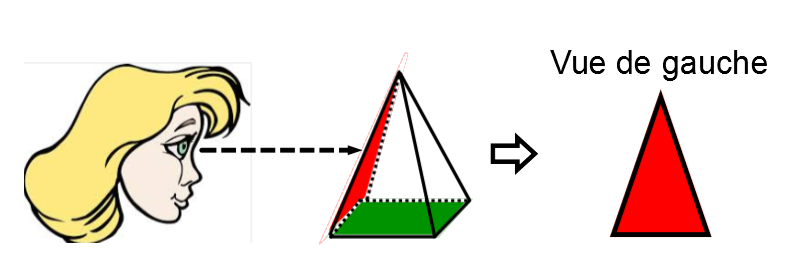
\includegraphics[width = 1\linewidth]{img/vueGauche.PNG}
            \caption[]{Visualiser le solide depuis la gauche}
        \end{figure}


    Exercices :

   \newpage
   \section{Vues coordonnées}
    Ci-dessous, on a les vues de face, de haut et de gauche de la pyramide
        \begin{figure}[H]
            \centering
            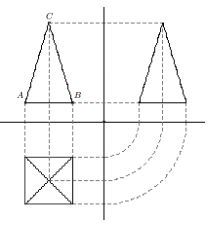
\includegraphics[width = 0.6\linewidth]{img/coordo.PNG}
            \caption[]{Vues coordonnées d'une pyramide}
        \end{figure}

            \newpage
    Exercices :\begin{itemize}
        \item Représente les vues de face, de haut, de gauche et de droite de la pyramide L8 P6 H7 \vspace{1\baselineskip}
        \item Représente les vues demandées ci-dessous: \begin{figure}[H]
            \centering
            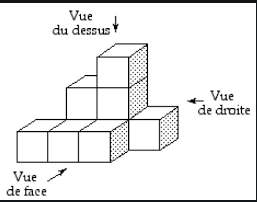
\includegraphics[width = 0.9\linewidth]{img/cubes.PNG}
            
        \end{figure}
        
    \end{itemize}
    
    
\end{document}
